\procTitle{Математическое моделирование для решения практических гидрологических задач на Северо-Востоке России}
\procAuthor{Нестерова~Н.\,В., Землянскова~А.\,А.}
\procEmail{nnesterova1994@gmail.com}
\procOrganization{СВНИМС ИМЗ СО РАН} \procCity{Магадан}

\makeProcTitle
\index{z@Землянскова~А.\,А.}
\index{n@Нестерова~Н.\,В.}

Ограниченность данных наблюдений за процессами формирования стока на Северо-Востоке России в современных условиях изменений климата является острой проблемой, решение которой позволит повысить надёжность проектирования и строительства в зоне распространения многолетнемерзлых грунтов. В ряде стран проблему нестационарности окружающей среды и низкой плотности гидрологической сети решают методами детерминированного гидрологического моделирования [6]. Таким образом, задача разработки научно-обоснованных, альтернативных методов оценок гидрологических характеристик рек зоны многолетней мерзлоты в условиях нестационарности окружающей среды, таких как методы моделирования, становится особенно актуальной в России.

Подавляющая часть гидрологических моделей, хорошо себя зарекомендовавших на территориях с умеренным климатом, не могут быть использованы для расчёта стока воды в зоне сезонного промерзания и распространения многолетней мерзлоты [1, 6]. В данной статье приводится описание детерминированной гидрологической модели <<Гидрограф>>, разработанной Ю.~Б.~Виноградовым в Государственном гидрологическом институте [1] и~развиваемой коллективом автором под руководством О.~М.~Макарьевой (добавить ссылки). Модель <<Гидрограф>> позволяет рассчитывать характеристики стока в бассейнах рек зоны распространения многолетней мерзлоты.

Модель содержит в себе алгоритмы, описывающие динамику тепла и~влаги в почвенном профиле в явном виде (рис.~1). Использование в качестве входной информации ограниченного числа метеорологических переменных (температура и влажность воздуха, осадки) позволяет применять модель на~малоизученных бассейнах. Результатами моделирования является не только сток воды в замыкающем створе, но и распределенные переменные состояния ландшафтов~--- характеристики снежного покрова, температура и~влажность почвы на разных глубинах, глубина протаивания и~промерзания, глубина залегания грунтовых вод и др., что позволяет проводить многокритериальную валидацию результатов расчётов на их соответствие наблюдаемым процессам и явлениям.

Для оценки параметров в пределах исследуемых бассейнов выделяются однородные природные зоны, так называемые стокоформирующие комплексы (СФК), по которым производится систематизация параметров модели. СФК~--- часть территории речного бассейна, условно однородная по~свойствам ландшафта, и единообразно функционирующая в гидрологическом плане. Предполагается, что все параметры модели характеризуют СФК в целом, неизменны в его пределах и скачкообразно изменяются на~его границах. Разнообразие почвенно-растительного покрова в сочетании с~рельефом создают условия формирования стока воды [1]. Для выделения СФК производится анализ сочетаний различных типов почвы, растительности и топографических условий [5]. Параметры модели представляют собой физические свойства почв и растительности, которые могут быть измерены в полевых условиях или оценены на основе описания ландшафтов и их характеристик. Поэтому при использовании модели <<Гидрограф>> калибровка параметров сводится к минимуму или совсем не требуется [5]. Это свойство модели <<Гидрограф>> позволяет применять ее в задаче оценки изменений как гидротермического режима деятельного слоя, так и гидрологического режима бассейнов рек.

Гидрологическая модель <<Гидрограф>> в концептуальном виде учитывает наличие на водосборе различных бассейновых ёмкостей, имеющих характерное время истечения и объем, в том числе с характеристиками скоростей влагообмена до десятков и сотен лет. Разработанная Ю.~Б.~Виноградовым [1] концептуальная система стоковых элементов~--- иерархическая последовательность ярусов их расположения, принимающих участие в питании рек, основана на допущениях о том, что ёмкостные и фильтрационные свойства водовмещающих горных пород закономерно уменьшаются с глубиной залегания. Также уменьшается с глубиной и интенсивность истечения подземных вод в речную сеть с одновременным увеличением запасов воды в~подземных горизонтах. Система стоковых элементов также предполагает, что при увеличении площади бассейна увеличивается количество дренируемых горизонтов подземных вод, а <<возраст воды>> (время, прошедшее от выпадения осадков до появления воды в русловой сети) в руслах рек может достигать десятков и сотен лет.

Модель имеет разработанный интерфейс (рис.~1) и свидетельство о государственной регистрации программы для ЭВМ (Свидетельство о государственной регистрации программы для ЭВМ №2018619084 <<Комплексная программа распределенной гидрологической модели ,,Гидрограф‘‘>>, правообладатель О.~М.~Макарьева, дата регистрации 30.07.2018).

Модель <<Гидрограф>> успешно применялась в условиях малых, средних и крупных бассейнов Российской Арктики, включая рр.~Лена, Индигирка, Яна и Колыма и др. [2, 3, 4, 5, 8].

\begin{figure}[H]
%\begin{changemargin}{-1.25cm}{0cm}
  \begin{center}
    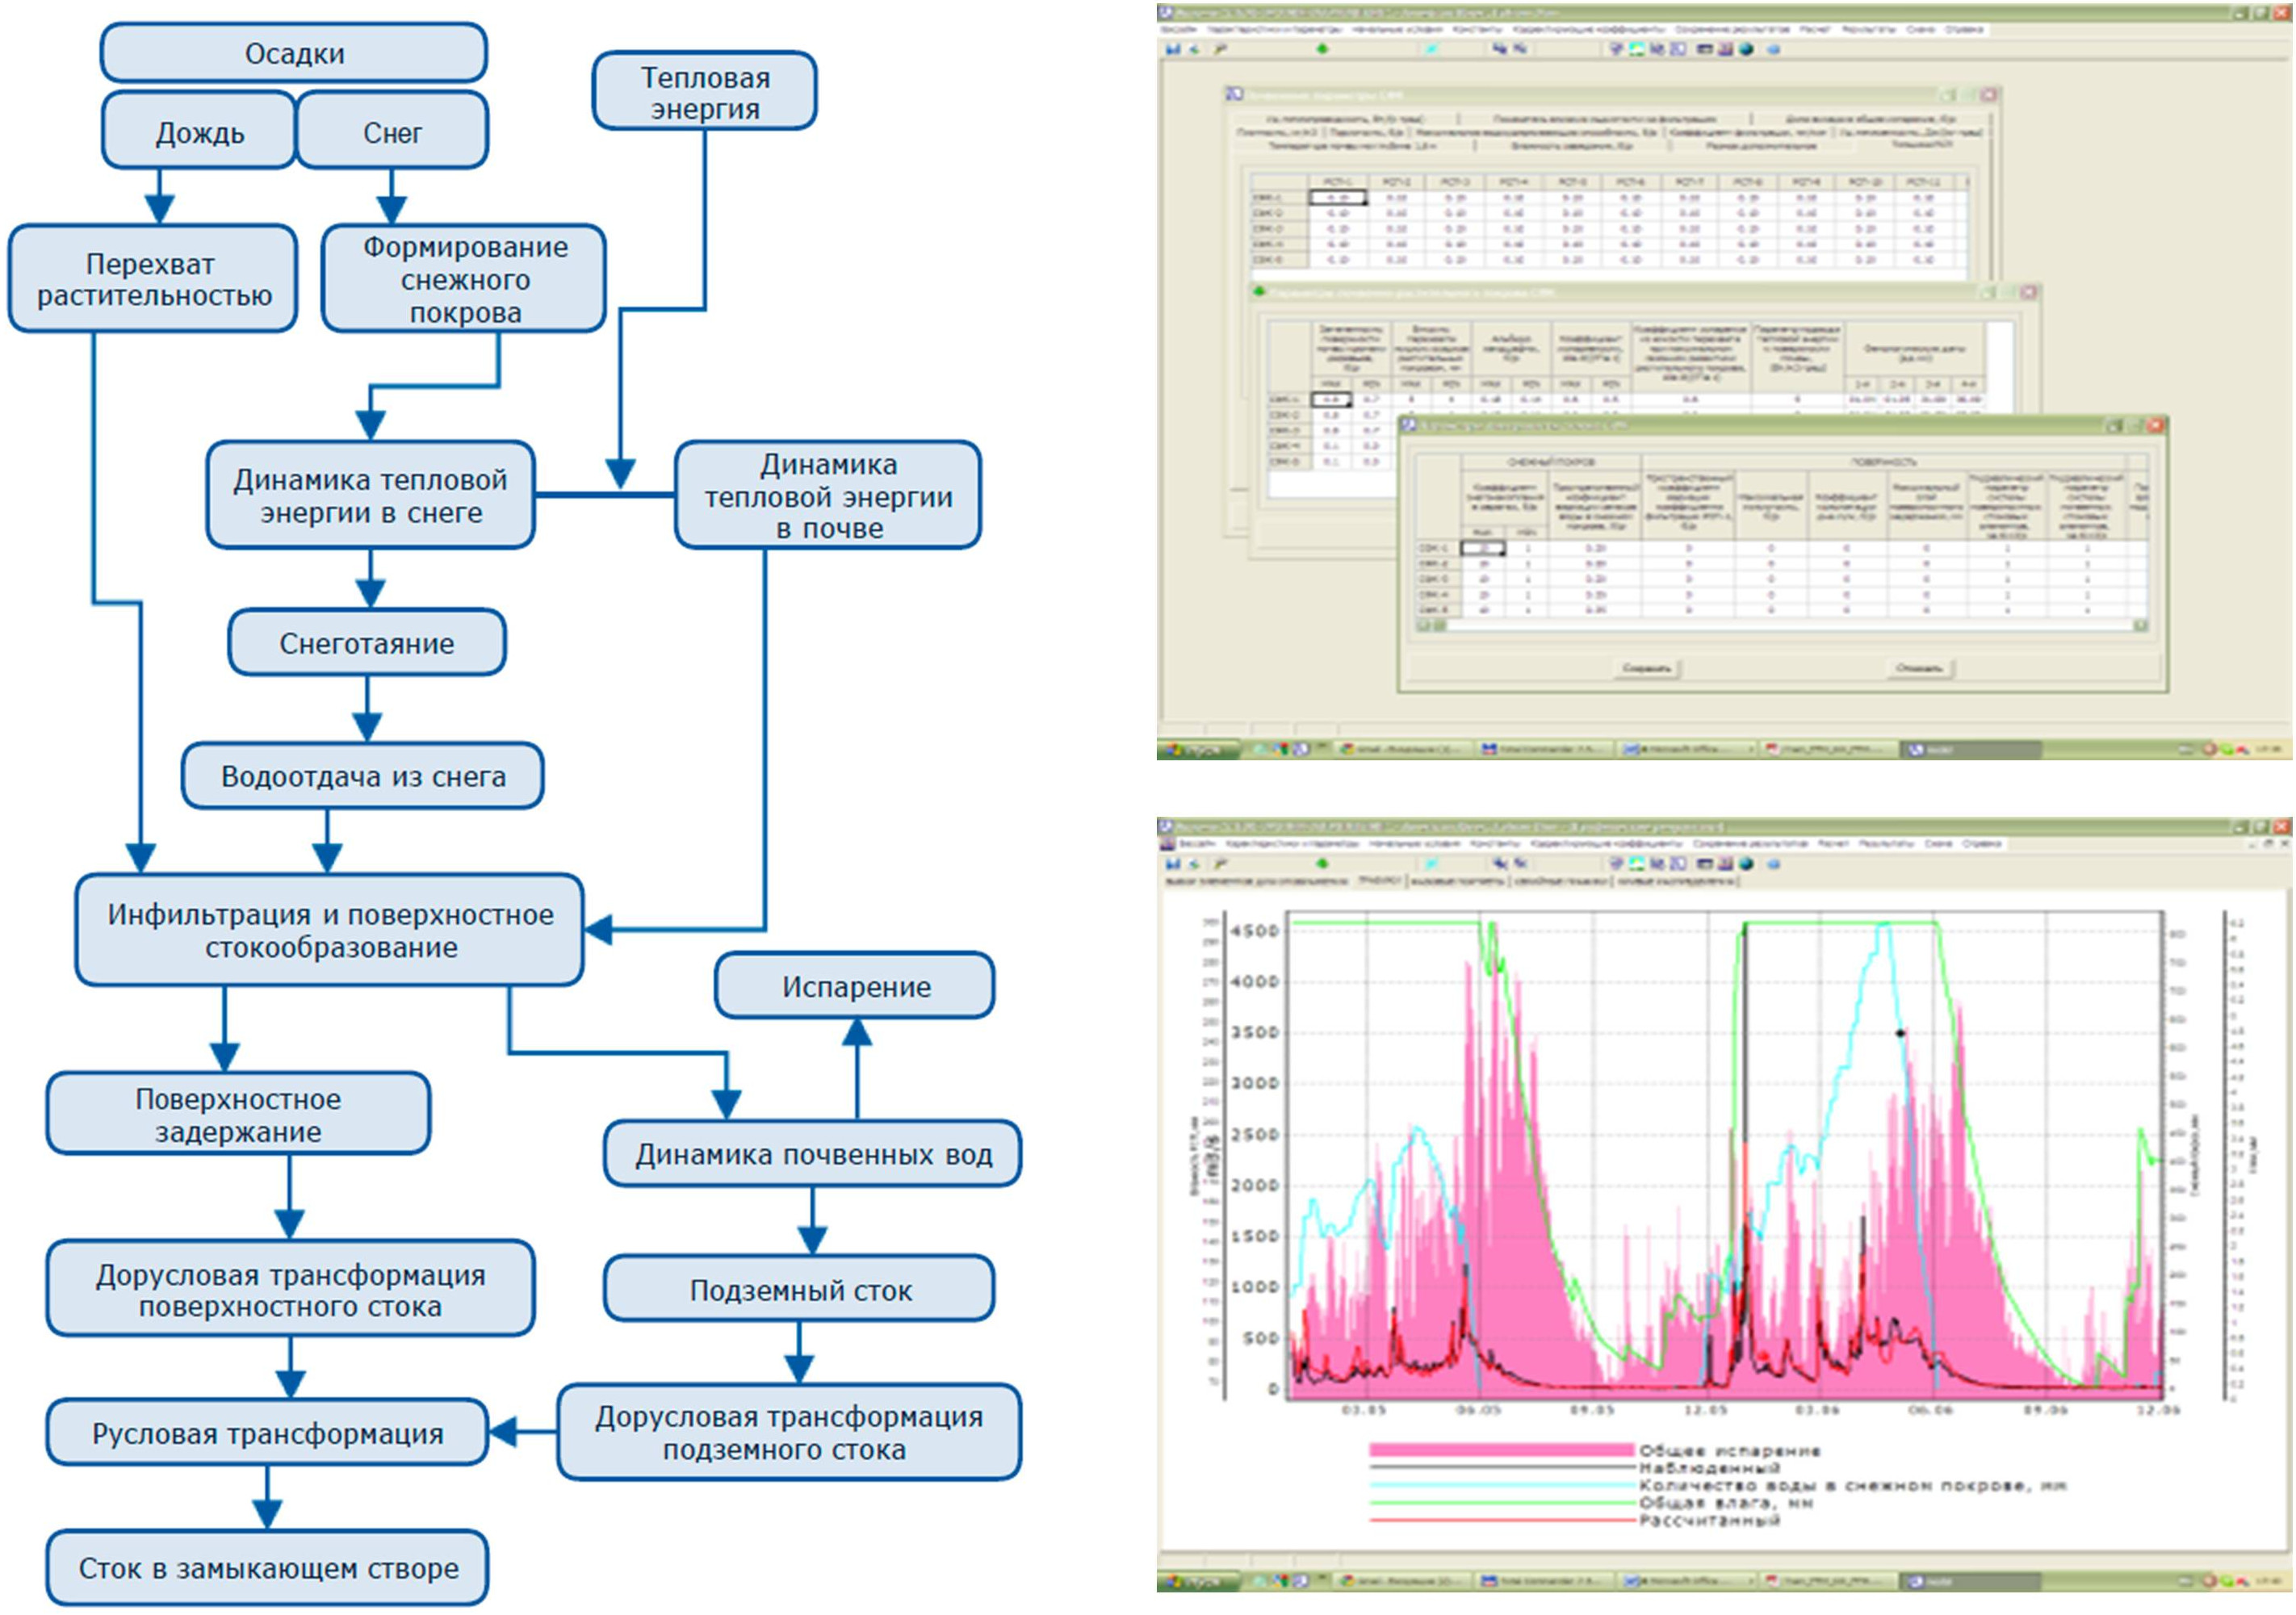
\includegraphics[width=1\textwidth]{authors/nesterova-1-fig-1.jpg}
  \end{center}
%\end{changemargin}
  \caption{Схема модели <<Гидрограф>> и её интерфейс}
  \label{fig:nesterova-1-fig-1}
\end{figure}


\textbf{Пример использования модели}

В качестве примера использования модели <<Гидрограф>> можно привести моделирование гидрологических процессов в басс.  р.~Сунтар~--- устье р.~Сахарынья [3]. В пределах данного водосбора в период 1957--1959~гг. функционировала Высокогорная станция Сунтар-Хаята, на которой проводились гляциологические, геоморфологические и геокриологические наблюдения в рамках программы Международного геофизического года. На~основе данных наблюдений и описаний ландшафтов и их характеристик разработаны параметры модели <<Гидрограф>> для гольцового ландшафта.

Согласно высотной поясности водосбор р.~Сунтар разбит на четыре стокоформирующих комплекса: гольцы, тундра, тайга, заболоченные редколесья и луговые болота. Для каждого комплекса разработана схематизация вертикального профиля, учитывающая состав грунта, растительность, процессы снегонакопления и стокоформирования. Проведена верификация параметров модели на основе сравнения рассчитанных и наблюденных характеристик переменных состояний, в том числе запаса воды в снежном покрове, температуры грунта на различных глубинах, величин протаивания и промерзания деятельного слоя почвы, испарения с ландшафтов. Результаты моделирования признаны удовлетворительными.

Затем выполнено непрерывное моделирование стока с суточным разрешением для бассейна р.~Сунтар в створе устье р.~Сахарынья за 1957--1964~гг. с использованием данных четырёх метеорологических станций (Сунтар-Хаята, Нижняя база, Агаякан, Восточная). В период с 1968 по 2012~гг. моделирование стока для р.~Сунтар происходило с использованием двух метеостанций (Агаякан, Восточная). Получены основные характеристики водного баланса за данные периоды моделирования, рассчитаны значения критерия эффективности Нэша-Сатклиффа (NS) и построены гидрографы стока (табл., рис.~2). Результаты моделирования стока за данный период можно признать удовлетворительными. Факторами, обусловливающими погрешность, следует признать низкую точность гидрометеорологических измерений и недостаточно полную оценку доли участия подземных горизонтов в питании рек.


\begin{table}[H]
  \vspace{-8pt}
  \caption*{\textbf{Характеристики водного баланса, р.~Сунтар~--- устье р.~Сахарынья}}
    \vspace{-4pt}
  \label{tab:nesterova-1-tab}
  \vspace{-10pt}
  \begin{center}
  \begin{tabular}{cccccccc}
 \toprule
  Период    & Yo  & Ys  & P   & E   & Qo   & Qs   & NS 			(av, med, $\frac{max}{min}$)  \\[2pt]
 \midrule
  1957--1964 & 180 & 199 & 344 & 143 & 1659 & 1200 & 0,75; 			0,75; $\frac{0,88}{0,40}$  \\[6pt]
  1966--2012 & 180 & 203 & 332 & 127 & 1910 & 1905 & 0,58; 			0,67; $\frac{0,87}{-0,90}$ \\
\bottomrule
  \end{tabular}
\end{center}
  \vspace{-8pt}
\textit{Примечание:} Yo и Ys~--- наблюдённый и рассчитанный среднемноголетний годовой слой стока,~мм; P~--- осадки,~мм; E~--- испарение,~мм; Qo и Qs~--- максимальный наблюдённый и рассчитанный расход,~м$^3$/с; NS av~--- среднее значение NS; max и min~--- максимальное и минимальное значение NS.
  \vspace{-8pt}
\end{table}


\begin{figure}[h!]
%\begin{changemargin}{-1.25cm}{0cm}
  \begin{center}
    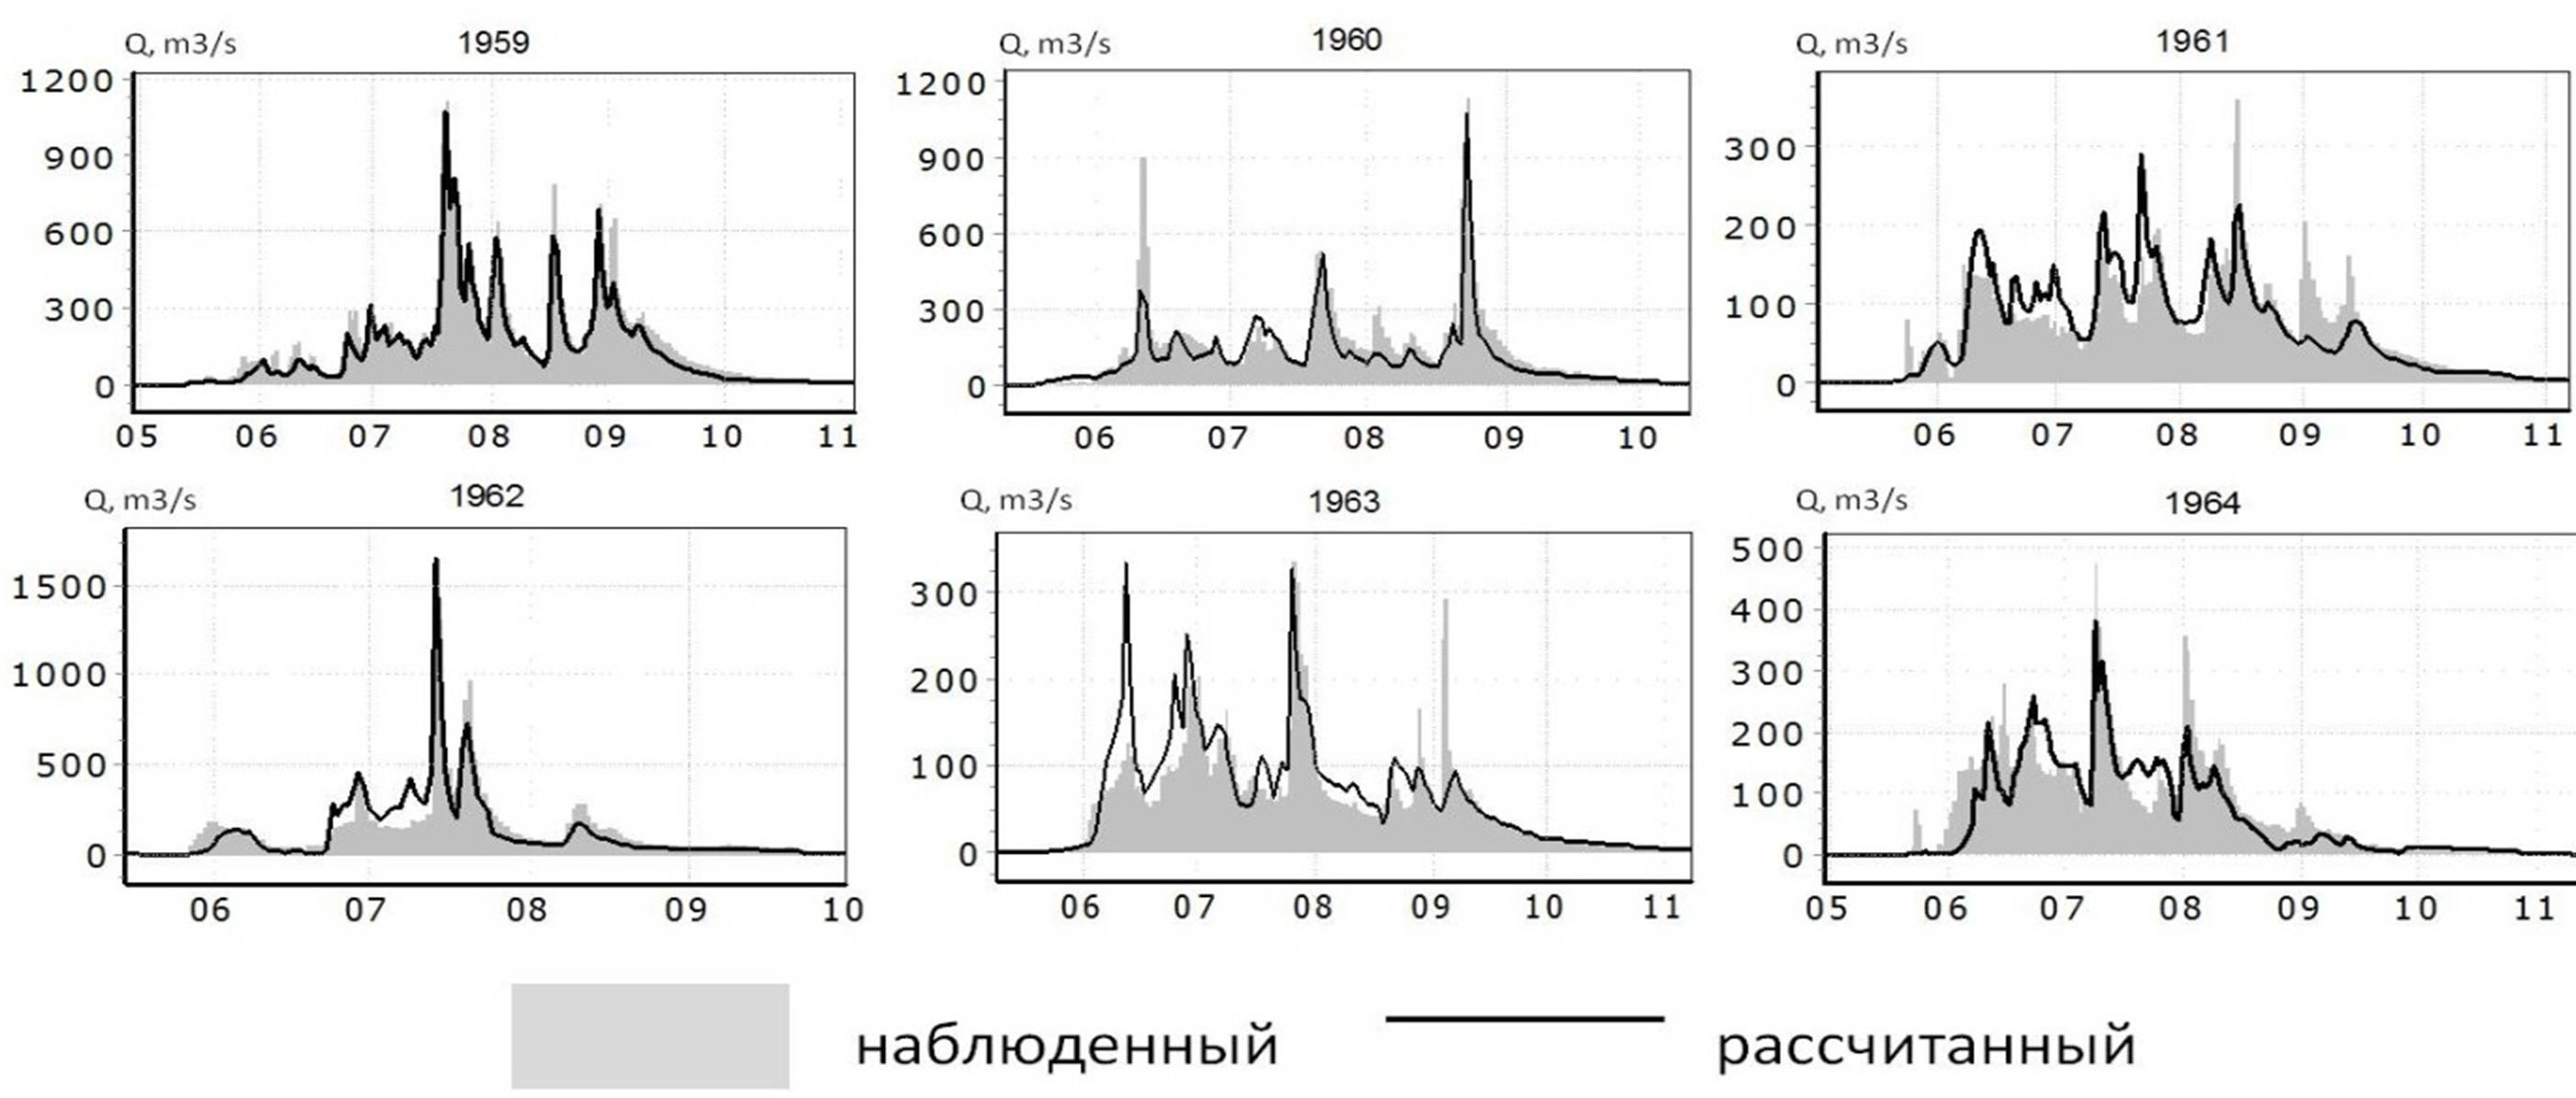
\includegraphics[width=1\textwidth]{authors/nesterova-1-fig-2.jpg}
  \end{center}
%\end{changemargin}
\vspace{-10pt}
  \caption{Рассчитанные и наблюдённые гидрографы стока, р.~Сунтар~--- устье
р.~Сахарынья, 1959--1964~гг.}
  \label{fig:nesterova-1-fig-2}
\vspace{-10pt}
\end{figure}
%\vspace{-10pt}


На основе результатов моделирования рассчитан вклад каждого СФК в~формирование стока в замыкающем створе. На гольцовый комплекс, занимающий 7\,\% территории водосбора, приходится 20\,\% общего стока в замыкающем створе р.~Сунтар, а коэффициент стока достигает 0,92. Наибольший вклад на формирование стока водосбора р.~Сунтар вносят тундры с~долей стока 49\,\% и коэффициентом стока 0,75. Суммарный сток с ландшафтов тайги и заболоченных редколесий, занимающих 56\,\% территории, составляет около 31\,\%.

В настоящее время, в горных районах басс. рр.~Яны, Индигирки и~Колымы не осталось ни одной исследовательской станции для комплексного изучения процессов формирования стока в различных ландшафтах мерзлоты. В этой связи все более актуальными становятся разработка и~верификация методов моделирования гидрологических процессов, применимых в~условиях крайней недостаточности информации. В работе показано, что гидрологическая модель <<Гидрограф>> может стать основой для решения научных и прикладных задач в исследуемом регионе.

Исследование выполнено при поддержке РФФИ~--- проект №~19-35-90090.

\begin{thebibliography}{99}
\bibitem{}\BibAuthor{Виноградов~Ю.~Б.} Математическое моделирование процессов формирование стока. Опыт критического анализа.~---  Л.~: Гидрометеоиздат, 1988.~--- 312~с.
\bibitem{}\BibAuthor{Лебедева~Л.~С., Семенова~О.~М., Виноградова~Т.~А.} Расчет глубины сезонно-талого слоя в условиях различных ландшафтов Колымской водно-балансовой станции в задаче гидрологического моделирования // Криосфера Земли.~--- 2015.~--- Т.~XIX, №~2.~--- С.~35--44.
\bibitem{}\BibAuthor{Макарьева~О.~М., Нестерова~Н.~В., Лебедева~Л.~С., Виноградова~Т.~А.} Моделирование процессов формирования стока рек высокогорной криолитозоны Восточной Сибири (на примере хребта Сунтар-Хаята) // География и природные ресурсы.~--- 2019.~--- №~1.~--- С.~178--186.
\bibitem{}\BibAuthor{Нестерова~Н.~В., Макарьева~О.~М., Виноградова~Т.~А., Лебедева~Л.~С.} Моделирование процессов формирования стока зоны Байкало-Амурской магистрали на основе данных полигона <<Могот>> // Водное хозяйство России.~--- 2018.~--- №~1.~--- С.~18--36.
\bibitem{}\BibAuthor{Lebedeva~L., Semenova~O., Vinogradova~T.} Simulation of active layer dynamics, Upper Kolyma, Russia, using the Hydrograph hydrological model // Permafrost Periglacial Process.~--- 2014.~--- Vol.~25.~--- P.~270--280.~--- DOI:~10.1002/ppp.1821.
\bibitem{}\BibAuthor{Lindström~G., Pers~C.~P., Rosberg~R., Strömqvist~J., et~al.} Development and test of the HYPE (Hydrological Predictions for the Environment) model~--- A~water quality model for different spatial scales // Hydrology Research.~--- 2010.~--- Vol.~41.~--- P.~295--319.
\bibitem{}\BibAuthor{Makarieva~O., Nesterova~N., Lebedeva~L., Sushansky~S.} Water balance and hydrology research in a mountainous permafrost watershed in upland streams of the Kolyma River, Russia~: a database from the Kolyma Water-Balance Station, 1948--1997 // Earth Syst. Sci. Data.~--- 2018.~--- Vol.~10.~--- P.~689--710.~--- DOI:~10.5194/essd-10-689-2018.
\bibitem{}\BibAuthor{Semenova~O., Lebedeva~L., Vinogradov~Yu.} Simulation of subsurface heat and water dynamics, and runoff generation in mountainous permafrost conditions, in the Upper Kolyma River basin, Russia // Hydrogeology Journal.~--- 2013.~--- Vol.~21.1.~--- Р.~107--119.~--- DOI:~10.1007/s10040-012-0936-1.

\end{thebibliography}
